\section{Appendix C. Cluster morphology operator and HFF benchmark}

This appendix documents the preregistered cluster morphology operator used to compare a gravitational-lensing convergence field ($\kappa$; treated here as a response proxy) against an observational hot-gas tracer constructed from Chandra imaging. The benchmark dataset is two Hubble Frontier Fields (HFF) clusters (Abell 2744 and MACS J0416.1$-$2403) using public HFF lens-model products accessed via the Mikulski Archive for Space Telescopes (MAST) \citep{MAST2019}.

\subsection{Data provenance and scope}

\begin{itemize}
	\item $\kappa$ maps (multi-team lens models): HFF community lens reconstructions accessed from the MAST Frontier Fields HLSP archive \citep{MAST2019}.
	\item X-ray proxy (stacked Chandra \texttt{img2} maps): HEASARC-served \texttt{*\_full\_img2.fits.gz} image products were stacked into a common WCS grid and used as a morphology/centroid proxy for the hot intracluster medium (ICM) \citep{HEASARC2025,Weisskopf2002}.
\end{itemize}

For reproducibility, the X-ray proxy construction follows a lightweight procedure implemented in \texttt{toy\_models/make\_chandra\_xray\_map.py}: each \texttt{img2} image is divided by a scalar exposure keyword (\texttt{EXPOSURE}, with \texttt{LIVETIME}/\texttt{ONTIME} fallbacks), reprojected onto a common WCS grid, and combined as an exposure-weighted mean rate map.

Important limitation: this work does not perform event-level Chandra reduction (exposure map correction, background modeling, point-source masking, etc.) in CIAO \citep{Fruscione2006}. The X-ray product is therefore intended as a geometric locator of bright ICM structure for centroid comparisons, not a calibrated surface-brightness measurement.

\subsection{Preregistered morphology operator}

For each cluster, each $\kappa$ team model, and each ROI radius, we apply the same fixed operator to $\kappa$ and to the X-ray proxy map:
\begin{itemize}
	\item \textbf{Smoothing:} apply Gaussian smoothing with $\sigma = 8\,\mathrm{arcsec}$ independently to $\kappa$ and X-ray maps.
	\item \textbf{ROI restriction:} within a circular ROI (fixed ICRS center per cluster), compute pixel-intensity thresholds at the 99th, 97th, and 95th percentiles of the smoothed pixels.
	\item \textbf{Primary-blob selection:} for each thresholded map, select the largest connected component above threshold.
	\item \textbf{Centroid definition:} compute the unweighted mask centroid of that connected component.
	\item \textbf{Measured quantity:} record the $\kappa$--X-ray centroid separation in arcseconds.
\end{itemize}

This definition is intentionally simple and falsifiable: it is fixed across clusters, teams, and thresholds, with only the ROI radius swept to quantify footprint sensitivity.

\subsection{Robustness grid: multi-team systematics and ROI sensitivity}

We evaluate ROI radius $\in \{80^{\prime\prime}, 100^{\prime\prime}, 120^{\prime\prime}\}$ for each cluster across available HFF teams, and report both (i) cross-team spread at fixed ROI, and (ii) ROI sensitivity within each team model. The complete tables are in \texttt{toy\_models/HFF\_ALL\_TEAMS\_SYSTEMATICS\_ANALYSIS.md} and the per-team measurements are available from the author upon request.

At ROI $= 100^{\prime\prime}$, Abell 2744 shows a relatively stable median $\kappa$--X-ray separation ($\approx 66$--$67^{\prime\prime}$ across thresholds) with small cross-team interquartile ranges ($\approx 1$--$1.5^{\prime\prime}$) but with a nontrivial full range at high thresholds. MACS J0416.1$-$2403 shows much larger cross-team dispersion at higher thresholds (IQRs growing to tens of arcseconds), reflecting stronger lens-model dependence of the inferred morphology under this operator.

\begin{figure}[t]
	\centering
	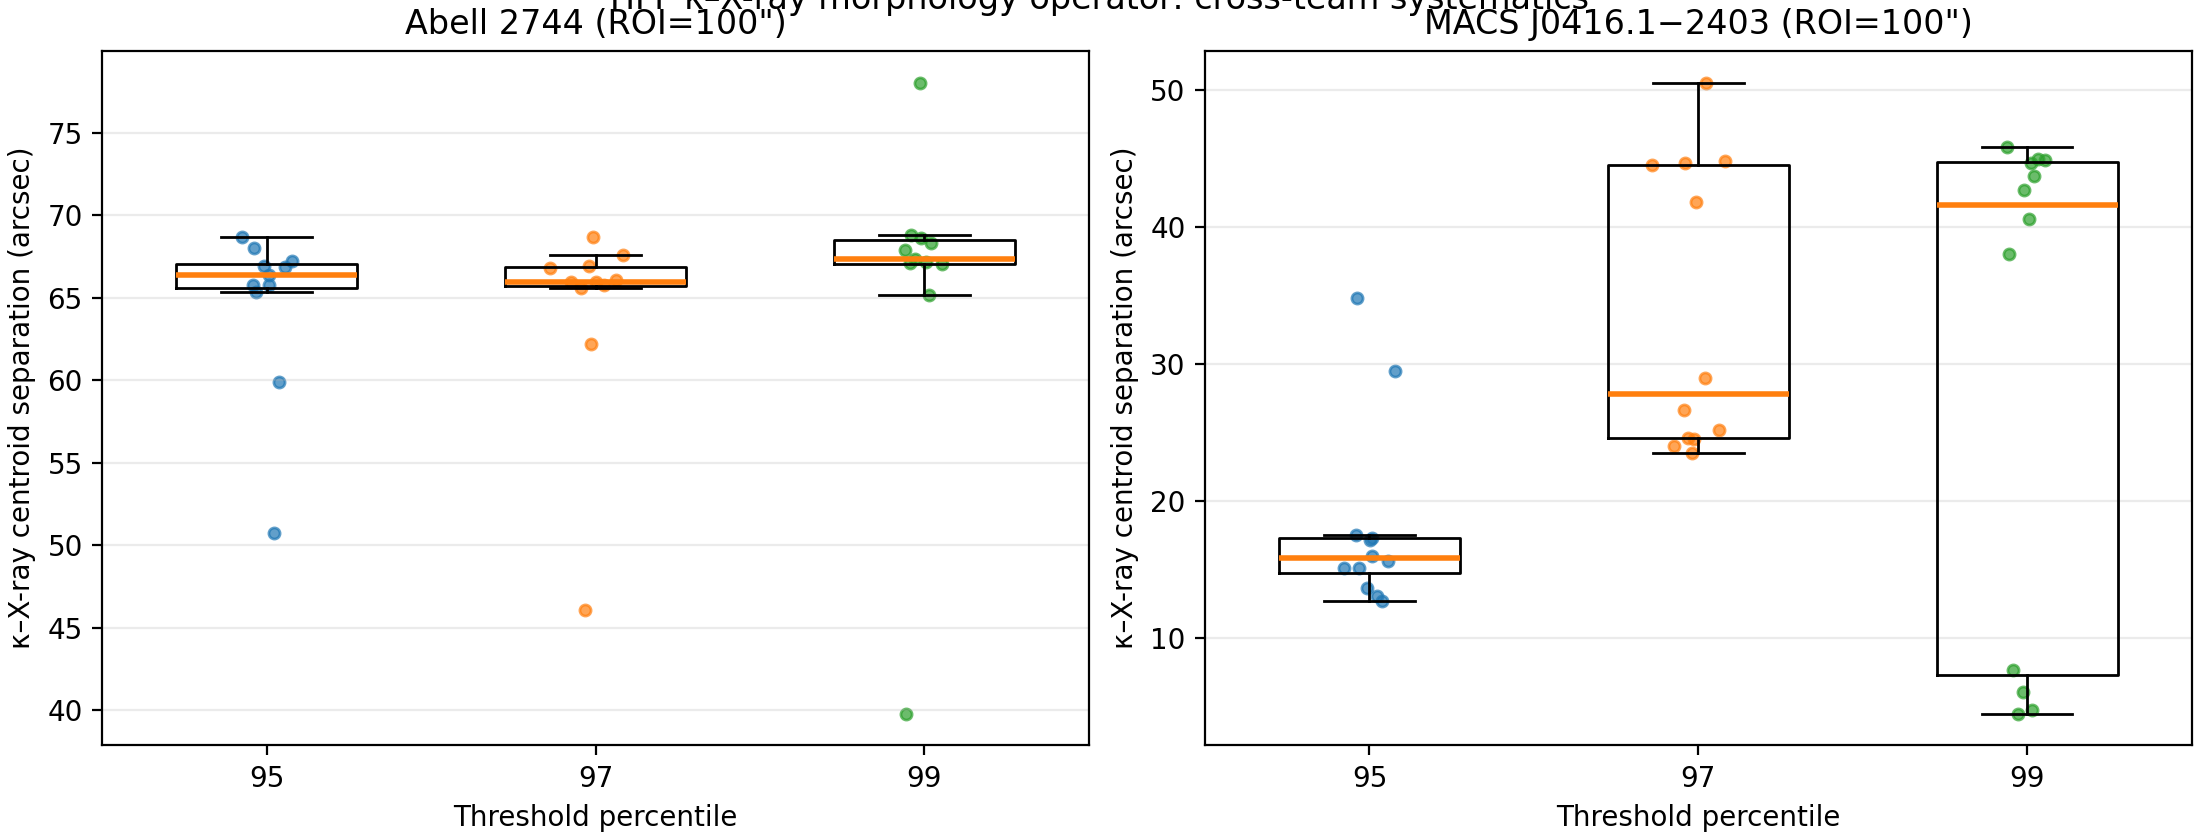
\includegraphics[width=\linewidth]{figures/hff_systematics_summary_roi100.png}
	\caption{HFF $\kappa$--X-ray systematics summary at ROI $=100^{\prime\prime}$ for Abell 2744 and MACS J0416.1$-$2403, showing cross-team dispersion under the fixed morphology operator across intensity thresholds.}
	\label{fig:hff-systematics-summary-roi100}
\end{figure}

\subsection{Six-panel diagnostic figures (ROI = 100″)}

For interpretability, we generated per-team six-panel diagnostics at ROI $= 100^{\prime\prime}$, including $\kappa$, X-ray proxy, threshold masks, and centroid overlays. Representative examples are shown below; the complete figure sets are available from the author upon request.

\begin{figure}[t]
	\centering
	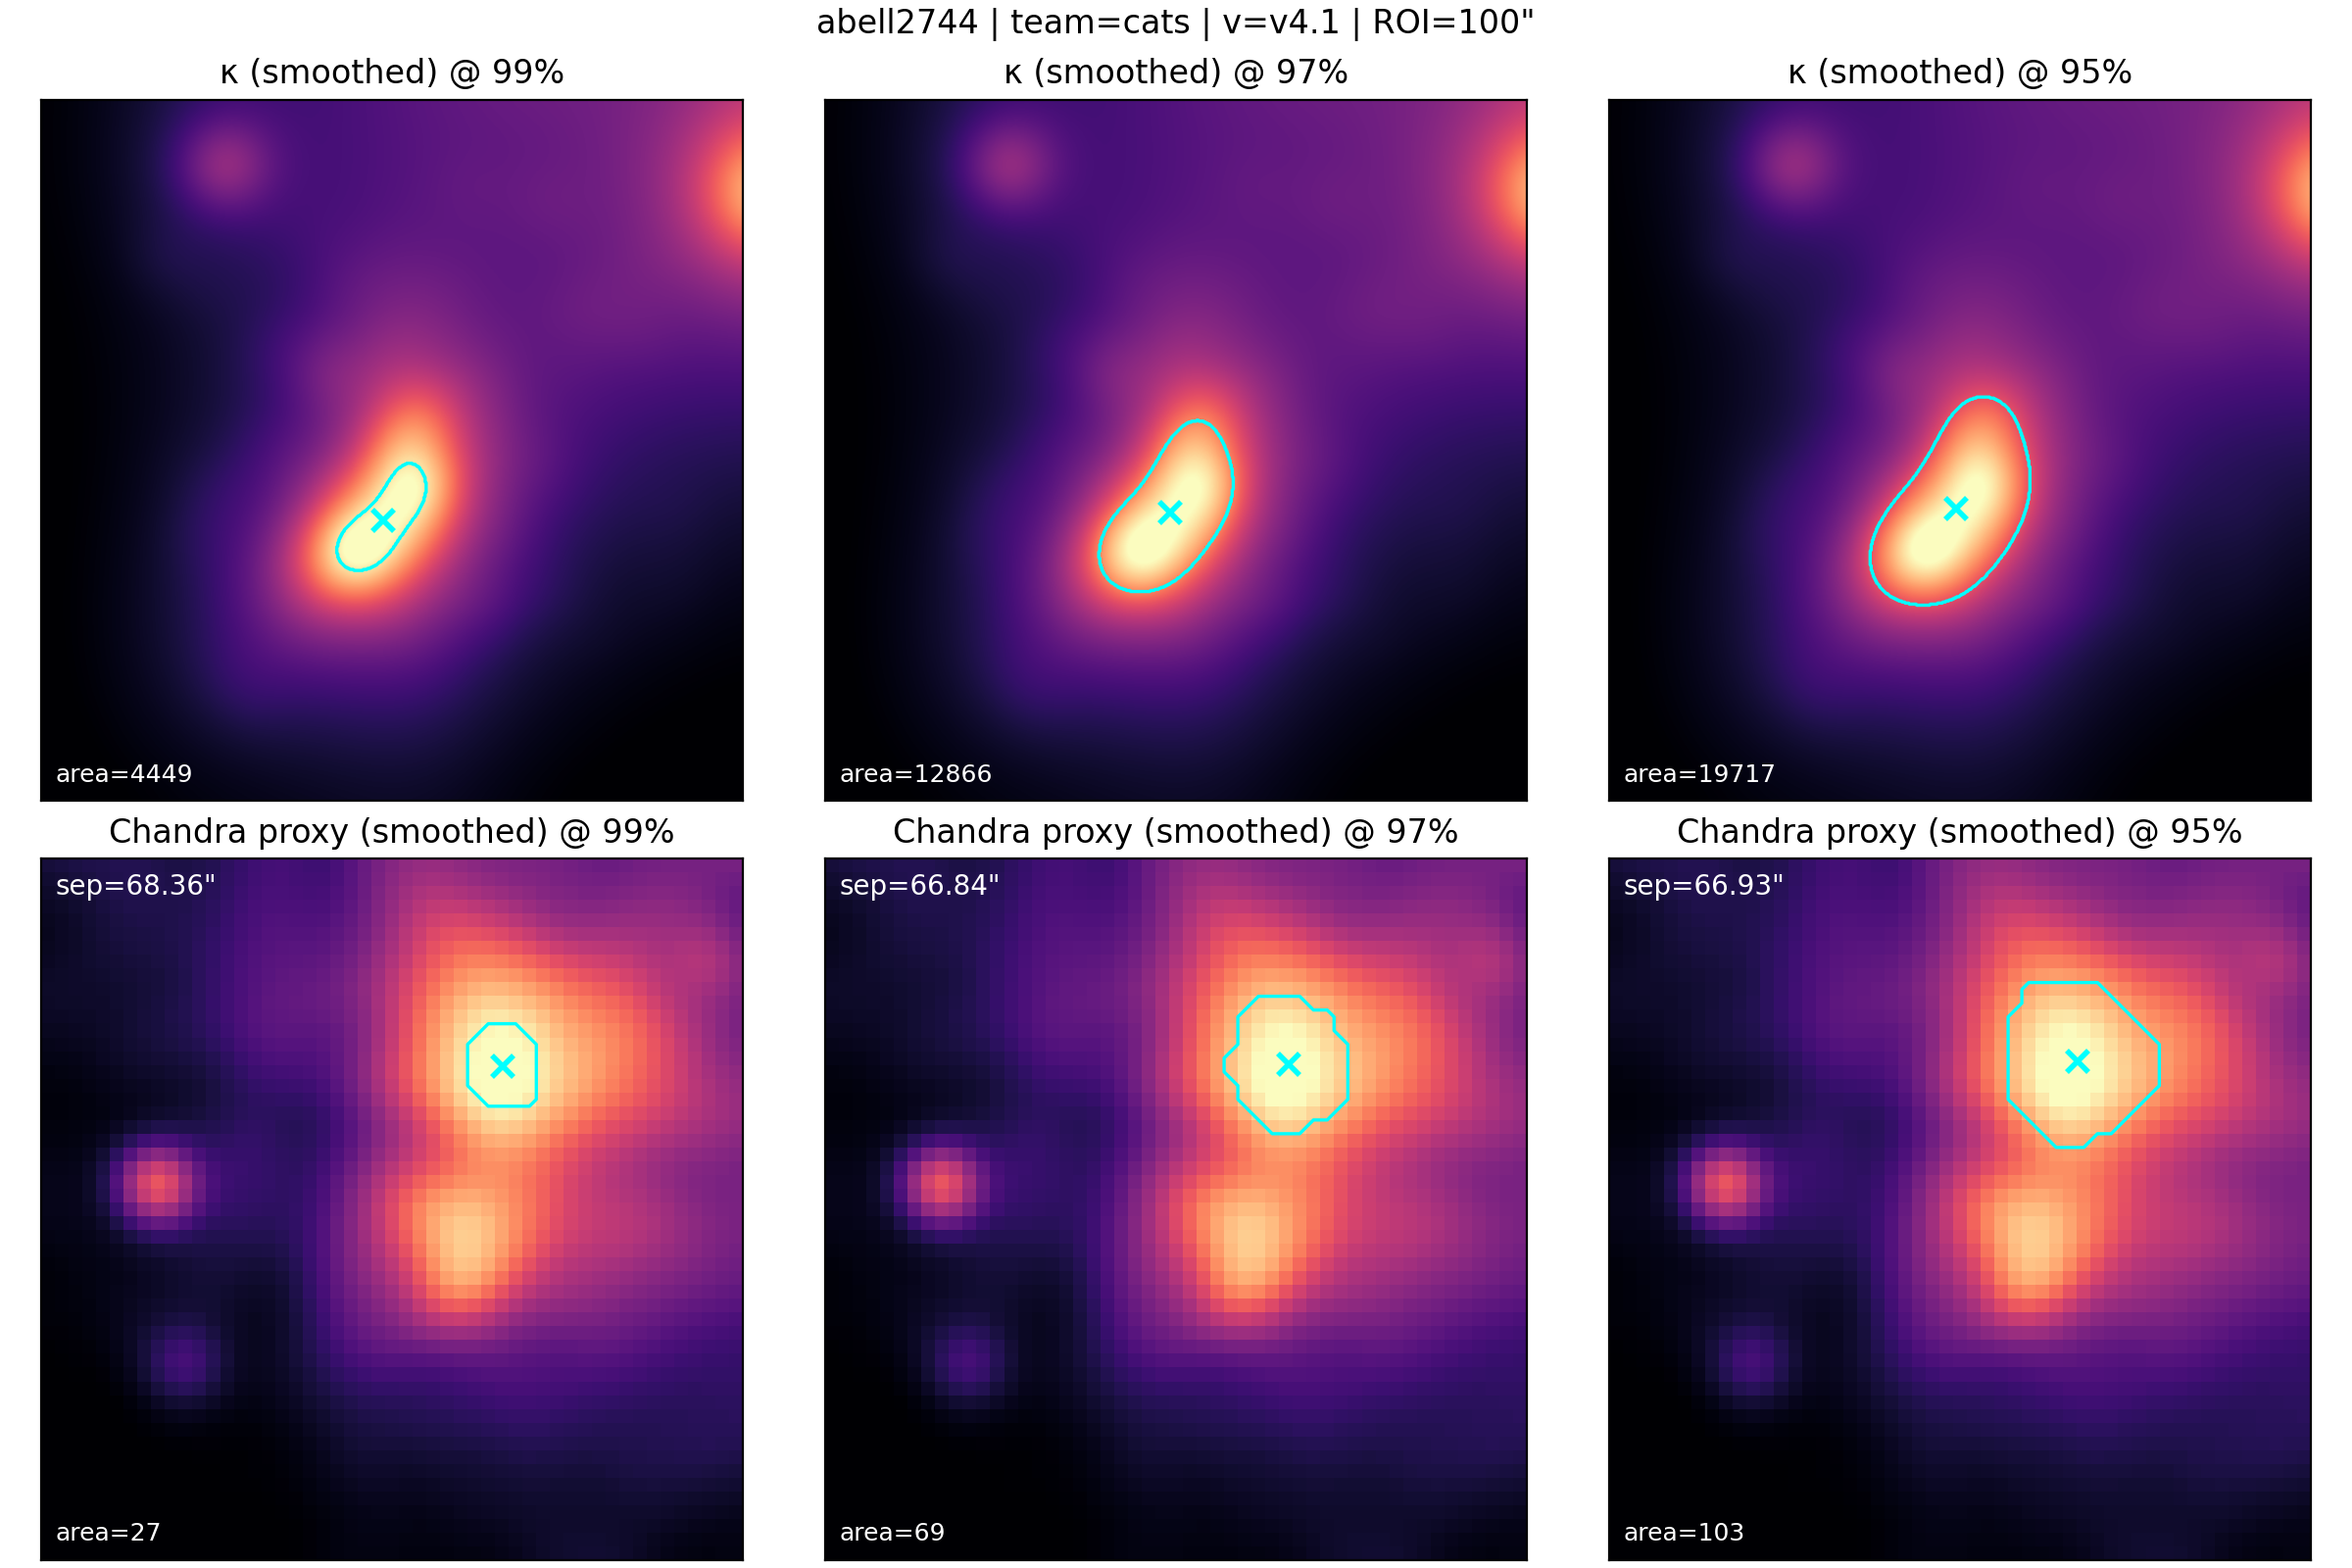
\includegraphics[width=\linewidth]{figures/abell2744_cats_v4p1_roi100_sixpanel.png}
	\caption{Six-panel diagnostic for Abell 2744 (CATS v4.1) at ROI $=100^{\prime\prime}$, illustrating the $\kappa$ field, X-ray proxy map, thresholded connected components, and centroid overlays used to compute the $\kappa$--X-ray separation.}
	\label{fig:abell2744-cats-v4p1-roi100-sixpanel}
\end{figure}

\begin{figure}[t]
	\centering
	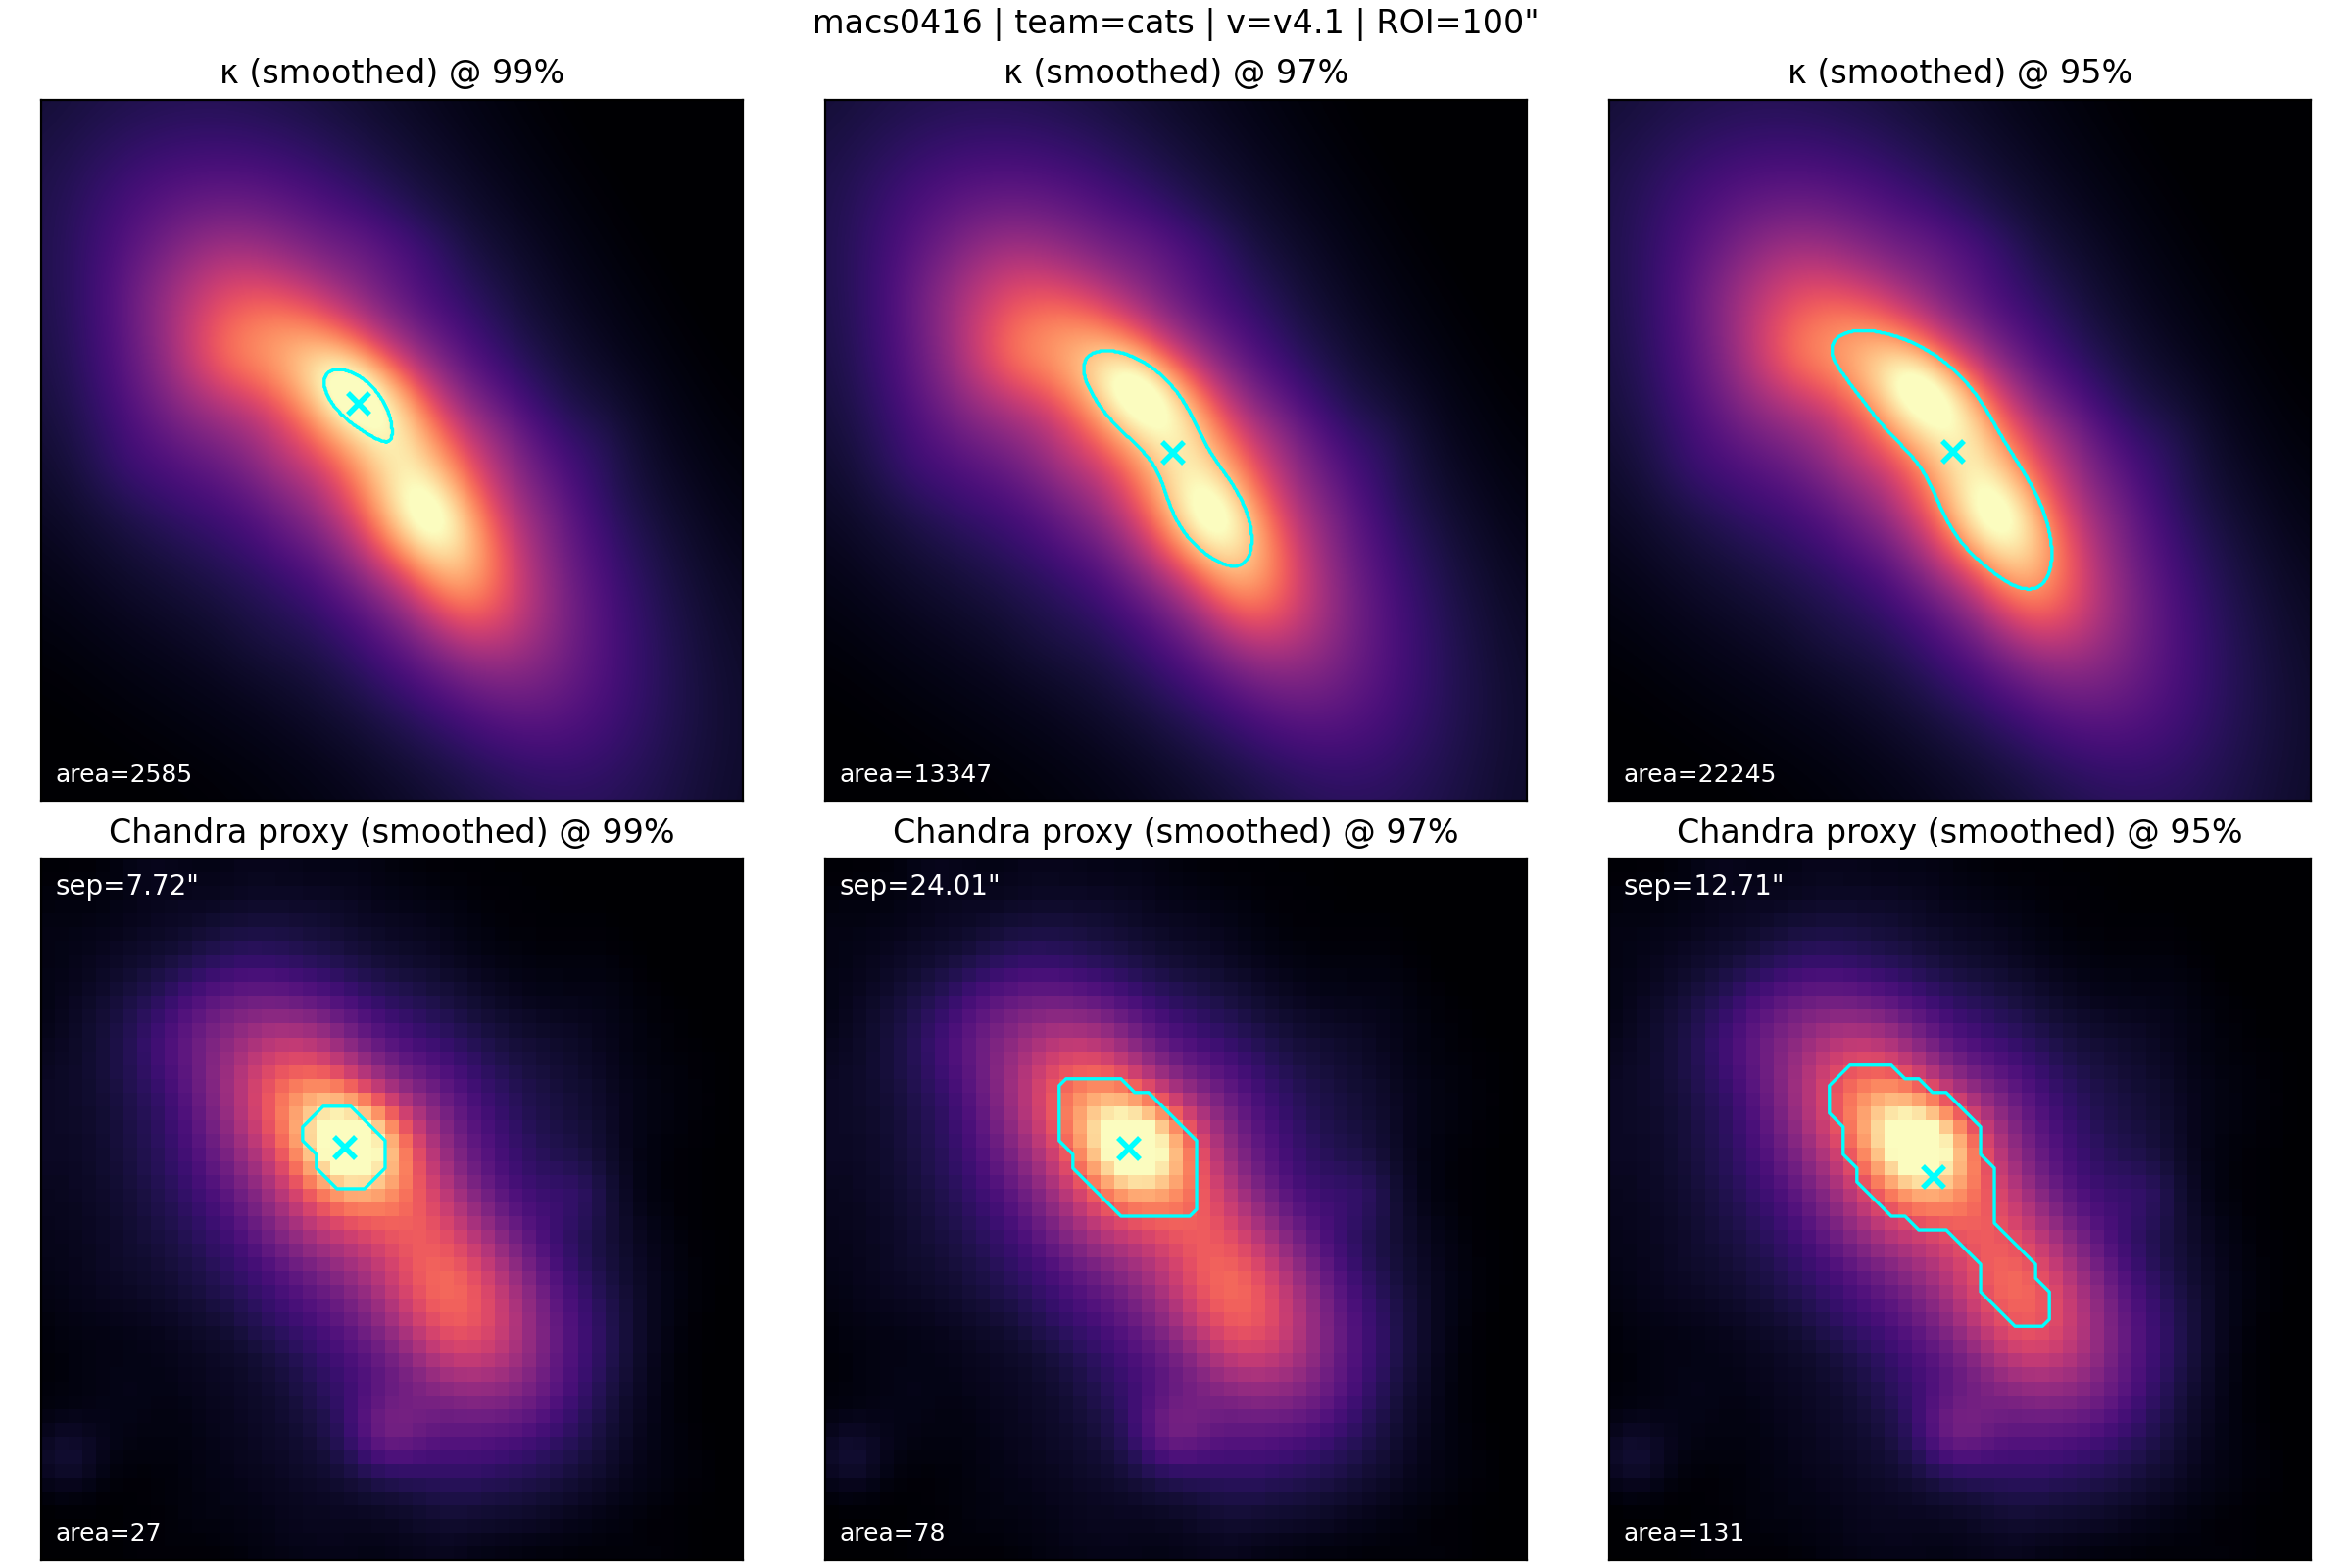
\includegraphics[width=\linewidth]{figures/macs0416_cats_v4p1_roi100_sixpanel.png}
	\caption{Six-panel diagnostic for MACS J0416.1$-$2403 (CATS v4.1) at ROI $=100^{\prime\prime}$, illustrating the $\kappa$ field, X-ray proxy map, thresholded connected components, and centroid overlays used to compute the $\kappa$--X-ray separation.}
	\label{fig:macs0416-cats-v4p1-roi100-sixpanel}
\end{figure}
